%!TEX root = thesis.tex

\chapter{Evaluation}
\label{chapter:evaluation}

In this chapter, I describe the evaluation of the tool built. I performed the evaluation by using two separate methods. I evaluated the efficiency of development process with the software effort and complexity metrics presented in chapter \ref{chapter:methods}. In addition, I evaluated the visualization effectiveness with heuristics by \citet{zuk_heuristics_2006} complemented by mapping objectives by \citet{schlichtmann_visualization_2002} presented in chapter \ref{section:visualizationprinciples}. As the first of the methods requires a baseline project, I decided to implement a number of sister projects as defined by \citet{kitchenham_evaluating_1998}. In this chapter, I refer to the visualizations built during sister projects with ``reference visualization'' and the visualizations built using Thematic.js with ``Thematic.js visualization''.

The most important findings of the evaluation are that 1) \emph{typically, Thematic.js improves the efficiency of building geographic visualizations significantly}, and 2) \emph{Thematic.js likely encourages creating effective visualizations}.

\section{Defining the Evaluated Cases}
\label{section:evaluatedcases}

The visualization tool should be able to visualize a large variety of data. Moreover, the benefits of reusable software are typically emphasized when examining a large number of relatively similar cases \citep{frakes_software_1996}. However, in order to keep the scope of this work manageable, I decided to evaluate a set of visualization cases listed below.

\paragraph{Alko stores in Finland}
Alko provides an unsupported representational state transfer (REST) API\footnote{\url{http://www.alko.fi/api/store/mapmarkers?language=fi}} for fetching data of Alko stores. The data is in a non-standard ``flat dot'' format (see appendix \ref{appendix:flatdotformat}). Therefore, I decided to visualize Alko store locations using a dot map. The resulting visualization should display all Alko stores in an effective fashion. The visualization should also provide clustering support for markers in order to avoid map cluttering. Figure \ref{fig:storemapresult} depicts the desired visualization result. This case is later referred to as ``store map''.

\begin{figure}[htbp]
  \begin{center}
    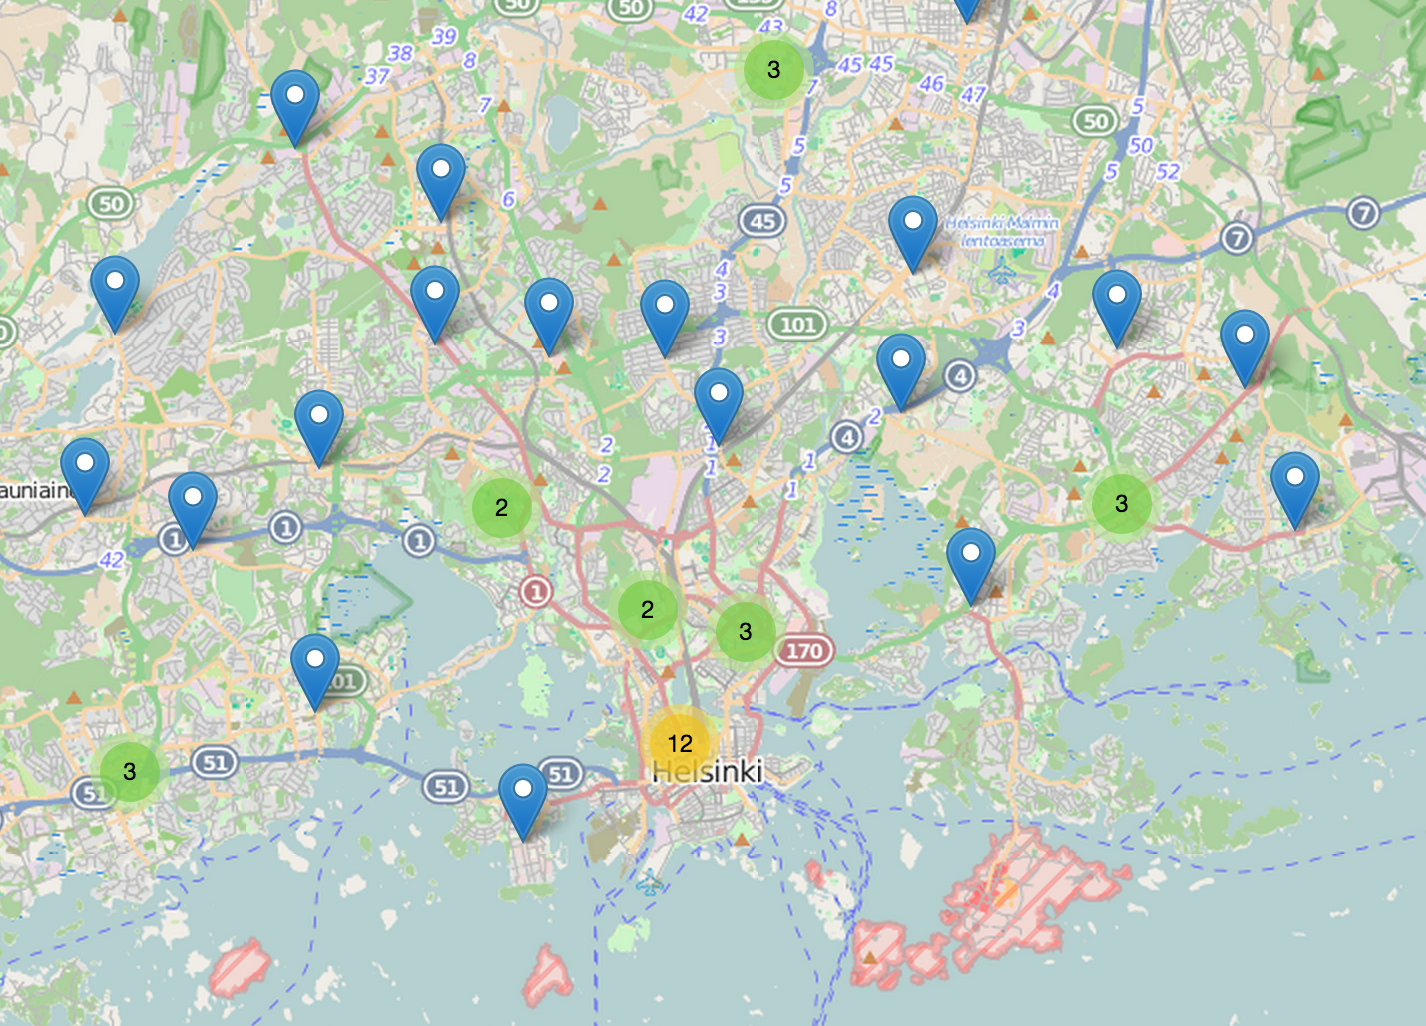
\includegraphics[width=8cm]{images/dotmap-example-thematic.png}
    \caption{A dot map depicting the desired result of the store map visualization.}
    \label{fig:storemapresult}
  \end{center}
\end{figure}

\paragraph{Earthquakes in California}
Earthquakes have two fundamental data axes: location and magnitude. Therefore, earthquakes are best visualized using a proportional symbol map with the size of the symbol representing magnitude. United States Geological Survey provides historical earthquake data\footnote{\url{http://earthquake.usgs.gov/earthquakes/search/}}, and I decided to visualize earthquakes in the state of California since January 1, 1900. The data is available in a Comma-Separated Values (CSV) format which is can be trivially transformed to ``flat dot'' JSON format. Figure \ref{fig:quakemapresult} depicts the desired visualization result. This case is later referred to as ``earthquake map''.

\begin{figure}[htbp]
  \begin{center}
    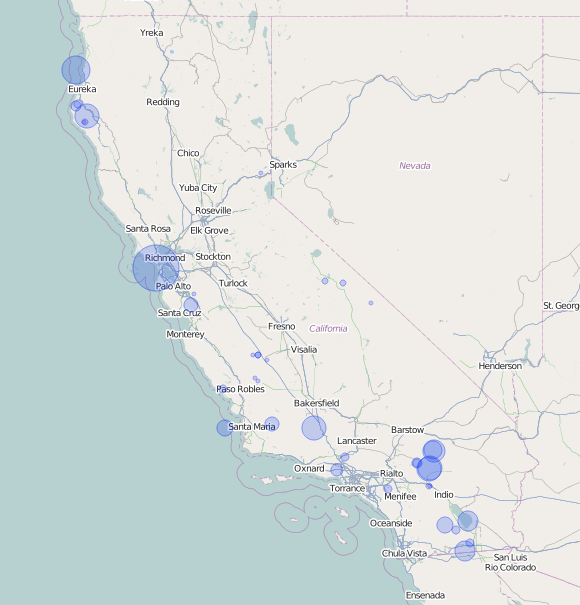
\includegraphics[width=8cm]{images/proportionalsymbol-example-thematic.png}
    \caption{A proportional symbol map depicting the desired result of the earthquake map visualization.}
    \label{fig:quakemapresult}
  \end{center}
\end{figure}

\paragraph{Voter Turnout in Finnish Presidential Election of 2012}
The Finnish Ministry of Interior provides regional voter turnout data of the presidential election of 2012\footnote{\url{http://tulospalvelu.vaalit.fi/TP2012K2/s/aanaktiivisuus/aanestys1.htm}}. This data is provided in electoral district and municipality level. I decided to visualize the turnout in municipality level, using municipality data by the Finnish Land Survey\footnote{\url{http://www.maanmittauslaitos.fi/en/opendata}}. The municipality data is provided in GeoJSON format by Teemu Tiilikainen\footnote{\url{https://github.com/varmais/maakunnat}}. The visualization should combine these data to create an effective choropleth visualization of regional turnout. The visualization should normalize the data in quantized fashion, i.e., using thresholds to create a discrete color range. Figure \ref{fig:voterturnoutresult} depicts the desired visualization result. This case is later referred to as ``election map''.

\begin{figure}[htbp]
  \begin{center}
    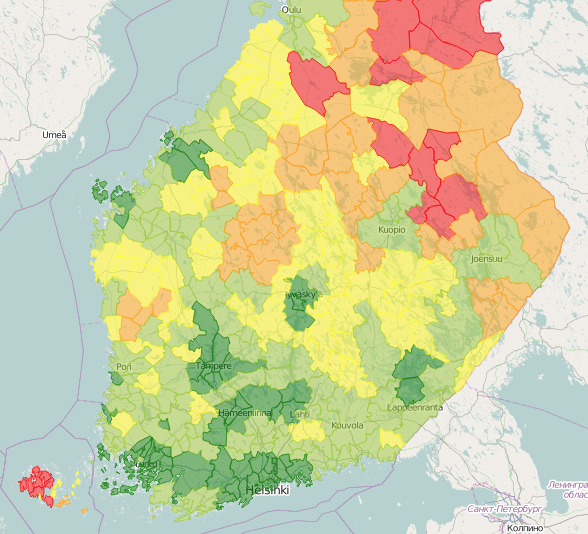
\includegraphics[width=8cm]{images/choropleth-example-thematic.png}
    \caption{A choropleth map depicting the desired result of the regional voter turnout visualization.}
    \label{fig:voterturnoutresult}
  \end{center}
\end{figure}

\paragraph{Share of People with No Secondary Education in Finland}
Statistics Finland\footnote{\url{http://www.tilastokeskus.fi/}} provides provincial data on the education of the population of Finland in CSV format. The visualization should combine this with province data by the Finnish Land Survey\footnote{\url{http://www.maanmittauslaitos.fi/en/opendata}} to create an effective choropleth visualization. The visualization should normalize the data in linear fashion, i.e., using a continuous color range. Figure \ref{fig:secondaryeducationresult} depicts the desired visualization result. This case is later referred to as ``education map''.

\begin{figure}[htbp]
  \begin{center}
    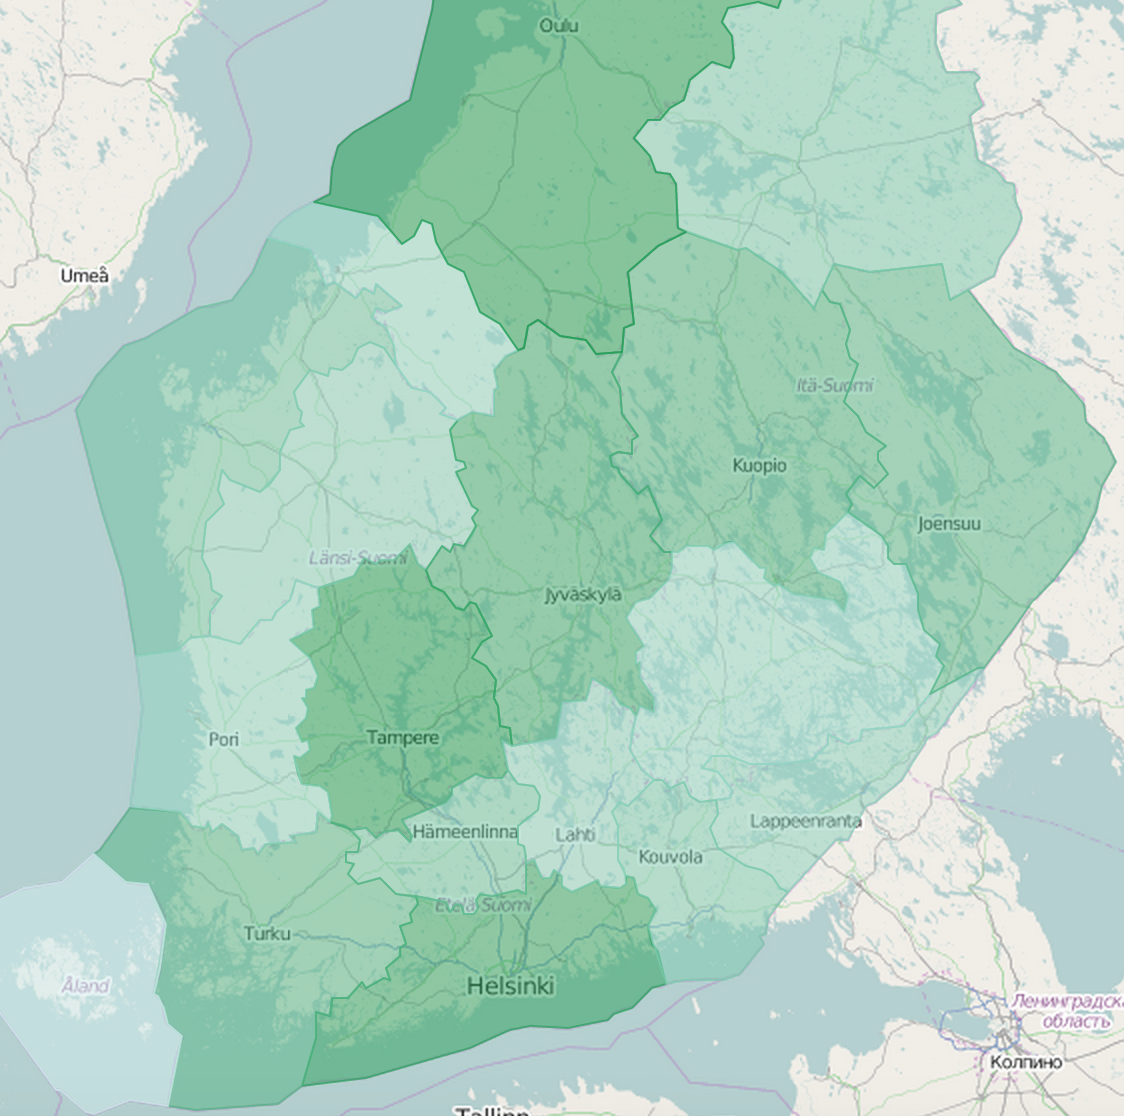
\includegraphics[width=8cm]{images/choropleth-d3-example.png}
    \caption{A choropleth map depicting the desired result of the secondary education visualization.}
    \label{fig:secondaryeducationresult}
  \end{center}
\end{figure}

\paragraph{Travel Times to a Single Destination}
Travel times to a destination can be visualized using an isarithmic map. I decided to visualize travel times to Futurice headquarters\footnote{\url{http://futurice.com/contact\#helsinki}} using public transport. The travel times can be obtained by using Travel Time Visualization Utility for HSL Reittiopas\footnote{\url{https://github.com/pyryk/reittiopas-travel-times}}. The utility provides the data in an approximated ``flat dot'' format. The visualization should normalize the data in a quantized fashion to emphasize isarithmic contours. Figure \ref{fig:isarithmicimpl} depicts the desired visualization result. This case is later referred to as ``simple travel times map''.

\begin{figure}[htbp]
  \begin{center}
    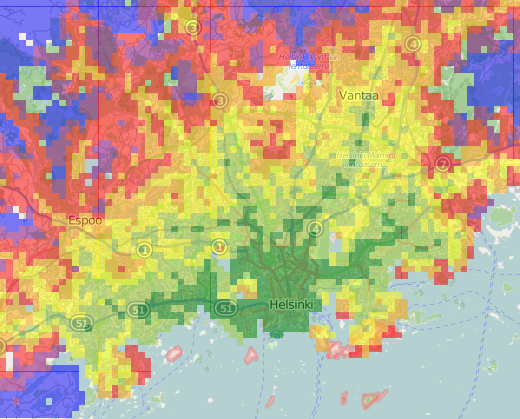
\includegraphics[width=8cm]{images/isarithmic-example-thematic.png}
    \caption{An approximated isarithmic map depicting travel times to Helsinki center.}
    \label{fig:isarithmicimpl}
  \end{center}
\end{figure}

\paragraph{Travel Times to Multiple Destinations}
In addition to visualizing travel times to a single destination, I decided to evaluate a case for displaying travel times to multiple destinations. The visualization should obtain the travel time data with the method defined in the previous paragraph, and combined using a weighted average method. Like in the previous case, the visualization should normalize the data in a quantized fashion. Figure \ref{fig:isarithmicimplcomplex} depicts the desired visualization result. This case is later referred to as ``complex travel times map''.

\begin{figure}[htbp]
  \begin{center}
    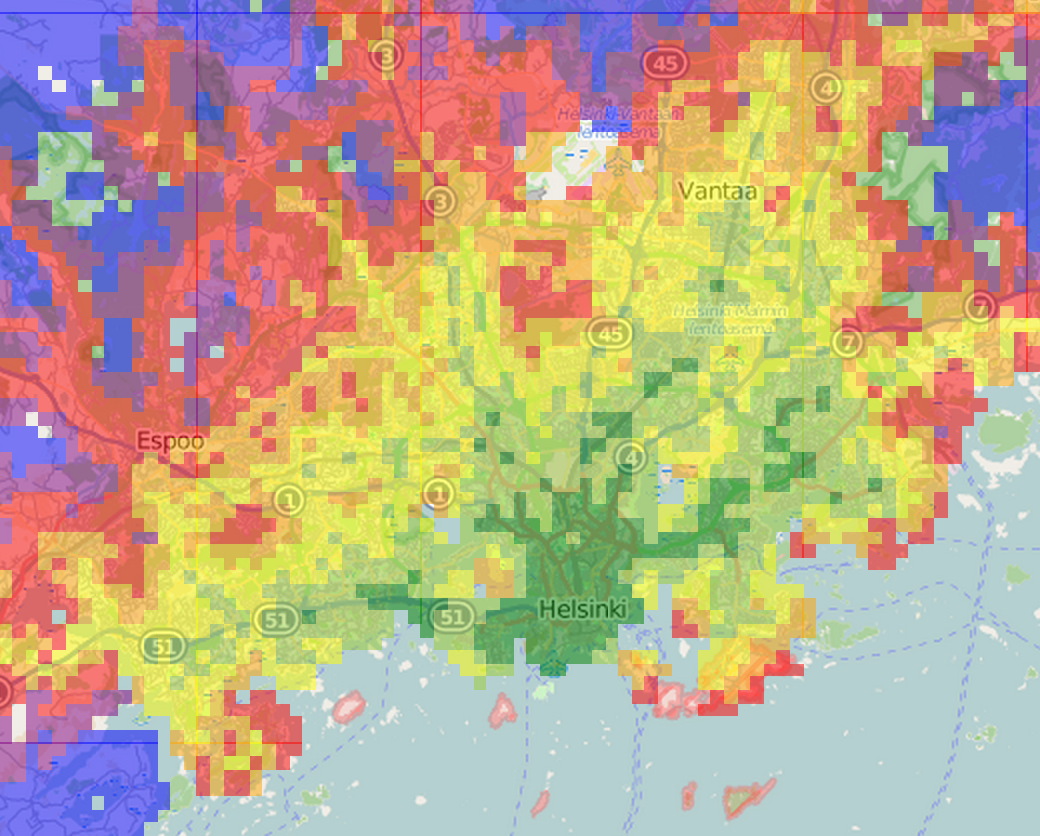
\includegraphics[width=8cm]{images/isarithmic-example-thematic-complex.png}
    \caption{An approximated isarithmic map depicting travel times to multiple destinations.}
    \label{fig:isarithmicimplcomplex}
  \end{center}
\end{figure}

~

While I selected the visualized data arbitrarily, I picked the cases to reflect the typical usage of visualizations. Choropleth map and isarithmic map are the most frequently used thematic mapping methods \citep[chap.~14-15]{slocum_thematic_2014}. Therefore, it is beneficial to the evaluation to examine multiple visualizations with those methods.

 The visualization cases include also a generic application structure and HTML features such as application caching and bookmarking support. These features are highly beneficial for web applications. I chose this approach in order to better model typical real-life use cases, and to be usable on the web.

\section{Implementing Sister Projects}

I implemented six separate sister project visualizations with no visualization library to compare to the visualization cases as defined in the previous section. The functionality of the visualizations was designed to reflect the functionality of the Thematic.js visualizations as accurately as possible. Sister visualizations were implemented using HTML, CSS and JavaScript to enable straightforward comparison to the evaluated visualization cases. I did not use any visualization library for the sister projects. However, I deemed using a generic mapping library such as Leaflet.js appropriate, because typically, creating map visualizations is not feasible without using one. Moreover, also Thematic.js uses Leaflet.js as a mapping library.

In order to better reflect the actual situations involving building visualizations, I implemented the sister projects in \emph{ad hoc} fashion. In practice, this means that I did not plan the design or architecture of the applications extensively beforehand. Also, I did not plan reuse of any form between visualizations. However, during implementation, I performed some design and code scavenging in order to speed up the development process. The sister project code is located in \url{https://github.com/pyryk/thesis-reference-implementations}.

\section{Evaluating Efficiency of Development}
\label{section:evaluatingefficiency}

I evaluated the efficiency of development by several metrics: software code length (number of physical (LOC) and logical (LLOC) lines of code), cyclomatic complexity (CC), Halstead difficulty (HD) and Halstead effort (HE). For measurements, I used ESComplex\footnote{\url{https://github.com/philbooth/escomplex}} for analyzing JavaScript programs. As the visualizations are implemented as single-page applications, the majority of the functionality lies within JavaScript. Only small part of the functionality involves HTML code and CSS definitions. Therefore, I decided to exclude HTML and CSS from the evaluation.

I began the evaluation by measuring the aforementioned metrics for the visualizations. It should be noted that for these measurements, I did not include code from Thematic.js or other third party libraries. The measurements are shown in table \ref{table:efficiencymetrics}.

\LTcapwidth=\textwidth
\begin{longtable}{|l|c|c|c|c|c|}
\hline
\textbf{Visualization} & \textbf{LOC} & \textbf{LLOC} & \textbf{CC} & \textbf{HD} & \textbf{HE} \\
\hline
\rowcolor{gray!15}
Thematic.js store & 12 & 12 & 1 & 7.31 & 4600 \\
\rowcolor{gray!15}
Reference store & 126 & 85 & 10 & 23.6 & 96500 \\
Thematic.js earthquake & 15 & 14 & 1 & 8.38 & 6280 \\
Reference earthquake & 79 & 121 & 10 & 23.5 & 87400 \\
\rowcolor{gray!15}
Thematic.js election & 26 & 29 & 2 & 10.9 & 12800 \\
\rowcolor{gray!15}
Reference election & 141 & 101 & 14 & 23.8 & 107000 \\
Thematic.js education & 17 & 17 & 1 & 10.2 & 10200 \\
Reference education & 129 & 87 & 10 & 27.8 & 109000 \\
\rowcolor{gray!15}
Thematic.js travel times simple & 27 & 28 & 2 & 10.8 & 9840 \\
\rowcolor{gray!15}
Reference travel times simple & 184 & 129 & 12 & 29.4 & 182000 \\
Thematic.js travel times complex & 30 & 30 & 2 & 11.6 & 13300 \\
Reference travel times complex & 193 & 144 & 12 & 34.5 & 255000 \\
\hline
\caption{Measurements for developed visualizations, including only visualization-specific code. The lower the value the better.}
\label{table:efficiencymetrics}
\end{longtable}

\emph{According to the results, using Thematic.js yields significantly lower complexity, difficulty and effort values when compared to using no visualization library.} This is likely a direct result of Thematic.js providing an extensive map-specific visualization functionality, allowing the visualizer to concentrate on the visualized data. In practice, this means that it is significantly more efficient to use a library such as Thematic.js than to write the map visualization from the ground up. 
% However, this conclusion assumes that the visualizer possesses -- or is able to achieve -- a general knowledge of the library functionality. % this is mentioned elsewhere and makes the sentence too long here

However, it is likely that the results do not describe the most typical real-life scenarios completely accurately. It can be assumed that typically, visualizers do not possess knowledge of Thematic.js functionality beforehand. Therefore, effort for each line of code is considerably higher than when building the visualization from the ground up. In the results, this is reflected in rather high values for relative difficulty for Thematic.js visualizations as seen in figure \ref{fig:evaluationchart}.
% passive, emphasizing ability (can be assumed) over actor (an evaluator)

\begin{figure}[htbp]
  \begin{center}
    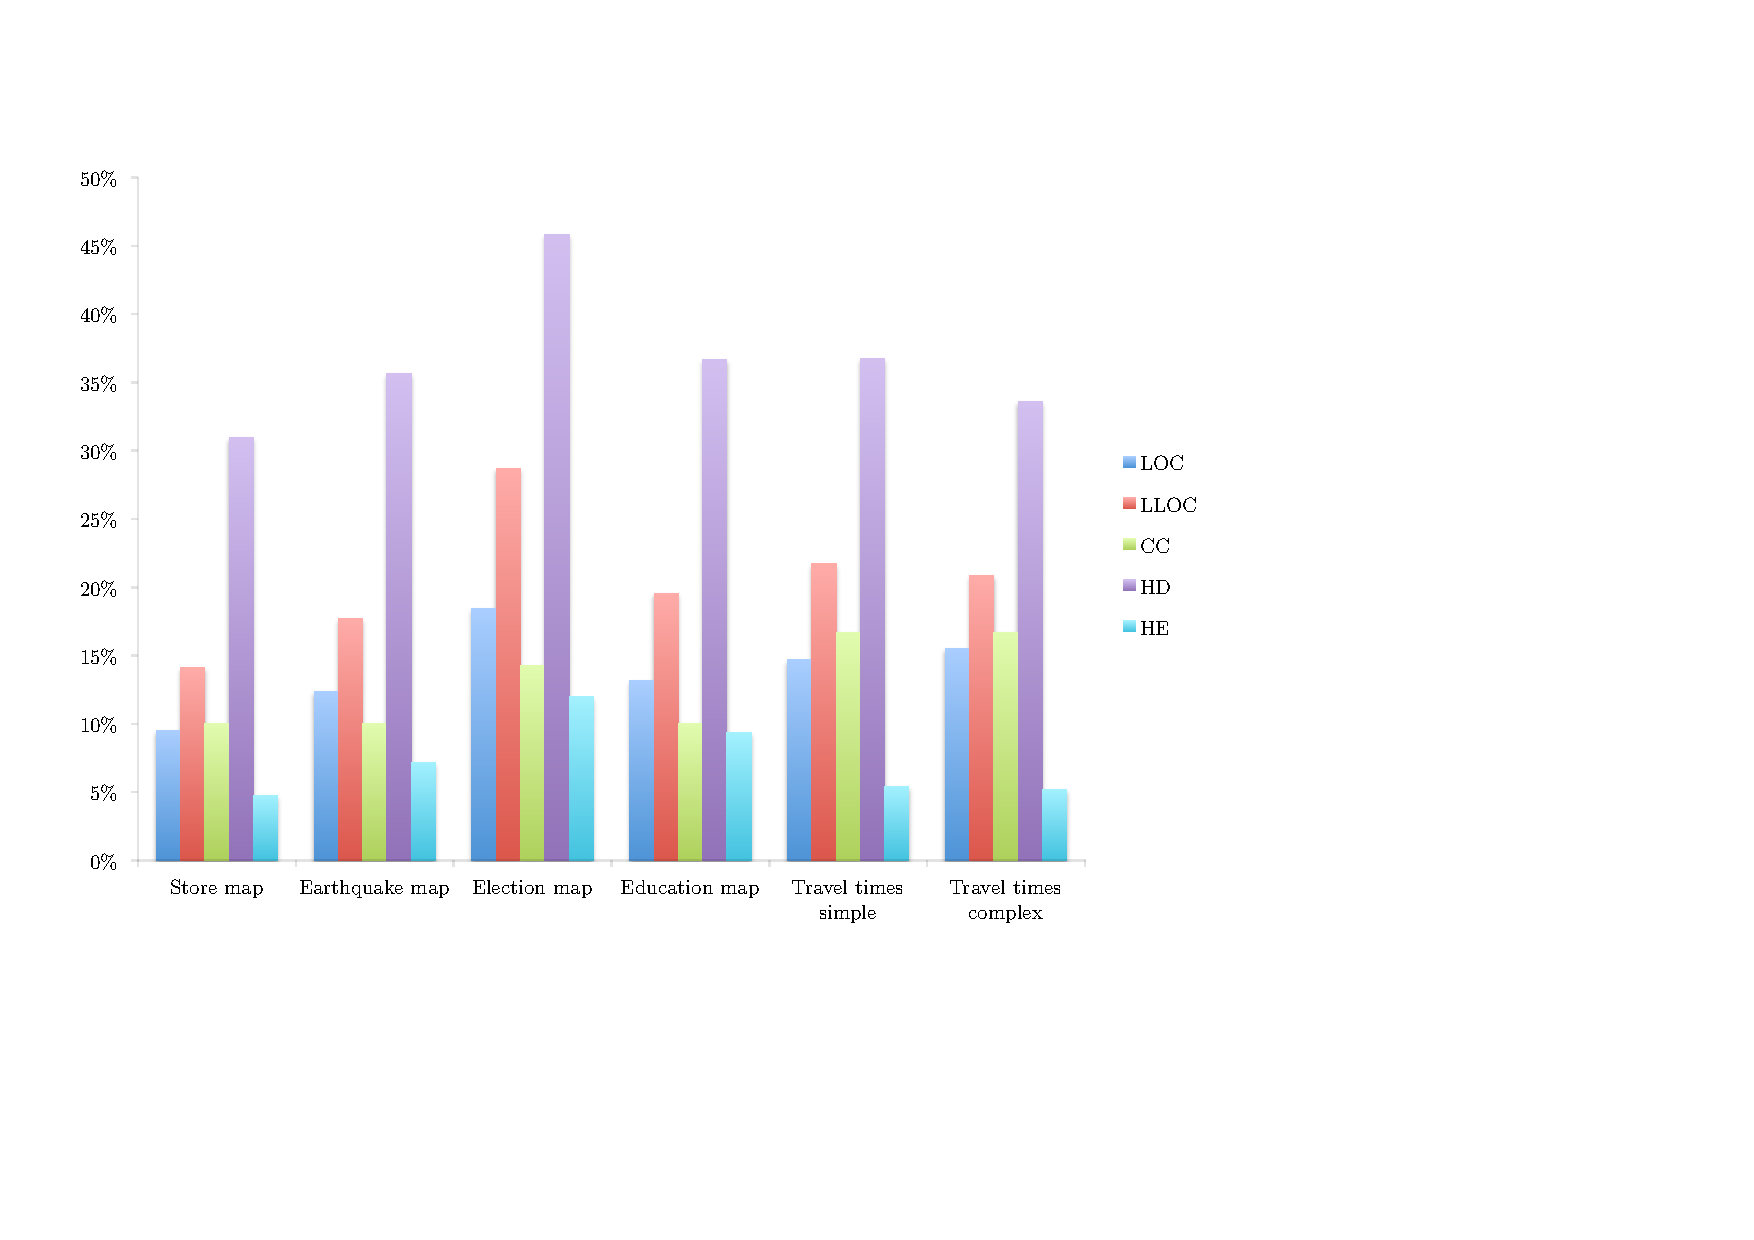
\includegraphics[width=\textwidth]{images/evaluation-results.pdf}
    \caption{Thematic.js visualization metrics for each case as a percentage of the corresponding reference visualization metric. The percentages are calculated using the values for each visualization case in table \ref{table:efficiencymetrics}}.
    \label{fig:evaluationchart}
  \end{center}
\end{figure}

Figure \ref{fig:evaluationchart} displays the ratio of Thematic.js visualization metrics for each visualization case to reference visualizations. I calculated these values using the determined absolute values for each visualization case as presented in table \ref{table:efficiencymetrics}. The resulting metrics provide a good overview of the effort needed for Thematic.js visualizations compared to using no visualization library.

Perhaps surprisingly, according to the results, using Thematic.js yields relatively high benefits for all metrics for the dot map visualization (store map). This may be surprising as dot map is an inherently simple mapping method. The reason for this may be that, e.g., error handling and marker clustering support add complexity to the reference implementation. Moreover, the Thematic.js visualization implementation for dot map visualization consists of only 12 lines of relatively simple code. Consequently, the boilerplate code needed in the reference implementation causes the relative metrics to be notably low.

Relative metrics of proportional symbol (earthquake) map are approximately similar to the metrics of dot map. However, the proportional symbol map is missing clustering support but involves symbol scaling functionality which is also needed in the Thematic.js implementation. Therefore, the relative metrics are slightly more favorable to the reference implementation than in the dot map case. Nevertheless, also in the proportional symbol case, using Thematic.js yields significant benefits compared to using no visualization framework. For example, Halstead effort measurement in Thematic.js implementation is under 10 \% of the corresponding measurement in the reference implementation.

Election map case yields the least benefits of all the evaluated cases. In this case, the Halstead difficulty is almost 50 \% and the Halstead effort over 10 \% of the value for the reference implementation. This is likely due to the fact that the Leaflet.js mapping library provides a comprehensive GeoJSON polygon support used with choropleth visualizations. Therefore, the additional manual implementation needed for the reference case is relatively straightforward. In this implementation, the most effort needed is related to the coloring and showing values. These features need to be implemented manually also in the Thematic.js implementation. That being said, even a simple choropleth map like this benefits considerably from the Thematic.js library.

In the education map case, using Thematic.js yields slightly greater benefits than in the election map. Like the election map, the education map uses choropleth mapping technique for visualization. However, the data in this case is already combined in GeoJSON format, so no manual combining is required. In both Thematic.js and reference implementations, an external coloring functionality is used, which reduces the size of the code bases. Especially the use of external coloring functionality reduces the Thematic.js relative complexity considerably. This results in more significant gains when using the library than in the election map case.

Both travel time maps yield highly similar results in measurements. This is likely due to the fact that both maps use isarithmic mapping method with relatively similar data. The only difference between the cases is the need for combining several data sources in the complex case. The data combining likely results in slightly lower values in Halstead difficulty and effort. However, in both of these cases, the Halstead effort metric is notably low. This indicates that the effort for visualizing with Thematic.js taking only 5 \% of the effort of the reference implementation. This is probably due to the fact that even approximated isarithmic visualization requires a complex graphics implementation not supported directly by any mapping library.

Across all cases, the Thematic.js measurements indicate more significant differences in physical lines of code than logical lines of code. This is likely due to the fact that I designed the Thematic.js API to encourage functional-style, chainable operations. Unlike in Thematic.js, traditional JavaScript APIs typically are imperative and non-chainable. The difference is demonstrated in listing \ref{listing:chainableapi}. Visualizers can use the chainable version without line breaks, resulting in only 1 physical line of code. With the API format in second example, it is not customary to combine the lines using only source code line. However, in practice, this has little effect on the actual effort needed as the underlying functionality stays largely similar.

\begin{lstlisting}[caption=Thematic.js API format. The code has been simplified to increase readability.,language=JavaScript,label=listing:chainableapi]
// chainable API supported by Thematic.js
map.addModule('voting', new Choropleth('percentage')
        .setScale(scale)
        .setData(data));

// non-chainable API typical for traditional
// JavaScript libraries
var module = new Choropleth('percentage');
module.setScale(scale);
module.setData(data);
map.addModule('voting', module);
\end{lstlisting}

Additionally, in all the cases, Halstead effort measurements in Thematic.js implementations are 4 to 12 \% of the reference implementations. However, corresponding Halstead difficulty measurements are 30 to 50 \% of the reference implementations. \emph{This reflects the fact that the reference implementations consist largely of straightforward but laborious boilerplate code such as initializing the map. Thematic.js implementations consist mostly of data-specific initialization of the visualization, which is typically less straightforward but considerably more concise.}

The results are statistically significant assuming the individual measurements are distributed normally. Using the dependent samples t-test, I determined that the difference in every evaluated metric is significant using the significance level of 1 \%.

Lastly, it should be noted that while the measurements are suitable for comparing different cases, as absolute metrics they are approximate at best. In practice, this means that it is not sensible to assume that using Thematic.js reduces the effort needed to 10 \% of the original. \emph{However, in light of these results, it seems extremely likely that using the library for visualizations similar to the evaluated cases yields considerable benefits over building the visualizations from the ground up.} For more details about the measurements, see appendix \ref{appendix:escomplex}.

\section{Evaluating Effectiveness of Visualizations}
\label{section:evaluatingeffectiveness}

In order to allow as reliable effort comparison as possible, I decided to implement the same functionality to reference visualizations as in Thematic.js visualizations. In practice, this results in the reference visualization being as similar feature-wise and visually to the Thematic.js visualization as possible. Therefore, it is not reasonable to compare the effectiveness of the corresponding reference and Thematic.js visualizations. Instead, I decided to evaluate the Thematic.js visualizations qualitatively, concentrating on how the library encourages the visualizer to create effective visualizations.

\emph{The results of the evaluation suggest that using Thematic.js may benefit the effectiveness of the visualization especially when used by inexperienced visualizers.} According to the evaluation, Thematic.js yields positive results related to 12 of the 25 visualization heuristics and 4 of the 10 objectives. The application yields negative results with only 1 of the 25 heuristics and none of the 10 objectives.

\subsection{Visualization Heuristics}

\citet{zuk_heuristics_2006} provide a list of 25 heuristics for data visualizations. I describe the heuristics in more detail in section \ref{section:visualizationprinciples}. I decided to use the heuristics as a basis for evaluating the created visualizations and Thematic.js functionality. I evaluated Thematic.js using a three-step scale for each heuristic. I deemed the result positive if the system has a positive effect (encourages conforming to the heuristic) when compared to using no visualization library. I deemed the result neutral if the system has no effect, and negative if the system encourages creating ineffective visualizations. I chose the approach to reduce the effects of the inherently subjective research method. With only three steps, the results are explicitly approximate but less likely to suffer from subjective evaluation. The evaluation results are outlined here. The full results, along with the reasoning, can be seen in appendix \ref{appendix:heuristicsevaluation}.

Almost all heuristics yield a nonnegative result. According to the results, Thematic.js yields a positive result (encourages the visualizer to conform to the heuristic) in 12 of the 25 criteria. Examples of these criteria are preserving action history and displaying details of the data on demand using popups. Using Thematic.js yields a neutral result (has no effect on conforming to the heuristic) in another 12 cases. I deemed only one case negative. In some cases, Thematic.js encourages the visualizer to unnecessarily increase graphical dimensionality by visualizing scalar data in a non-scalar fashion. In practice, this is the case when using the proportional symbol method. The overview of the heuristics evaluation can be seen in table \ref{table:heuristicsevaluationoverview}.

\begin{table}[htb]
\centering
\begin{tabular}{|c|c|c|}
\hline
\textbf{Positive} & \textbf{Neutral} & \textbf{Negative} \\ 
\hline
Size variation & Visual variable & Graphic dimensionality \\
Most data & Color order & \\
No extra ink & Color size & \\
Gestalt laws & Local contrast & \\
Levels of detail & Color blindness & \\
Integrate text & Preattentive benefits & \\
Overview first & Zoom and filter & \\
Details on demand & Relate & \\
Extract & Uncertainty & \\
History & Relationships & \\
Multivariate & Domain Parameters & \\
Hypotheses & Cause \& effect & \\
\hline
\end{tabular}
\caption{The overview of evaluation based on the 25 heuristics presented by \citet{zuk_heuristics_2006}.}
\label{table:heuristicsevaluationoverview}
\end{table}

\emph{The heuristics evaluation indicates that using Thematic.js may be beneficial to the effectiveness of the visualization. However, this is likely dependent on the visualizer.} An experienced visualizer will probably build visualizations which conform to the heuristics as well or even better without the library. However, for inexperienced visualizers, using the library is likely beneficial for building effective visualizations. 

\subsection{Thematic Mapping Objectives}

\citet{schlichtmann_visualization_2002} provide a list of objectives for thematic mapping. I cover the objectives in more detail in section \ref{section:thematicmaps}. I evaluated the Thematic.js library by examining whether the library encourages the visualizer to achieve the objectives or not. Like in the previous section with heuristics, I employed a three-step scale for evaluation. Result for each objective is regarded as \emph{positive} if the library encourages achieving the objectives better than a typical non-visualization mapping library does. Result is regarded as \emph{neutral} if using Thematic.js has no effect on achieving the objective, and \emph{negative} if Thematic.js discourages the visualizer to achieve the objective. I present the results in full detail in appendix \ref{appendix:objectivesevaluation}, with overview below.

Table \ref{table:objectivesevaluationoverview} displays the number of positive, neutral and negative results related to the objectives. I regarded the most of the results as neutral. This is likely due to the fact that many mapping libraries, such as Leaflet.js, already provide satisfactory level of support for many of the objectives. Therefore, using Thematic.js provides no additional benefit related to these objectives. Nevertheless, Thematic.js achieves a positive result for 4 out of 10 objectives. These are mostly due to providing explicit support for features encouraging effective visualizations, such as defining different symbols for different topeme types. It is also notable that I regarded none of the results as negative.

\begin{table}[htb]
\centering
\begin{tabular}{|c|c|c|c|}
\hline
\textbf{Positive} & \textbf{Neutral} & \textbf{Negative} \\ 
\hline
Clarification & Emphasis & \\
Types of entries & Sets of Types & \\
Cross-relations & Local syntax & \\
Addable and non- & Local ensembles & \\
addable quantities & Multilocal ensembles & \\
& The surface illusion & \\
\hline
\end{tabular}
\caption{The overview of evaluation based on objectives presented by \citet{schlichtmann_visualization_2002}.}
\label{table:objectivesevaluationoverview}
\end{table}

\emph{Thematic mapping objective evaluation hints that using Thematic.js may be beneficial to the effectiveness of resulting visualizations}. However, as with the heuristics results, this does not imply that Thematic.js is beneficial for every visualizer. An experienced visualizer may not benefit from the library in terms of effectiveness. However, especially for less experienced visualizers who might not recognize the objectives by heart, Thematic.js is probably beneficial.
